\documentclass{article}

\usepackage{graphicx}
\usepackage{float}
\usepackage{amssymb}
\usepackage{amsmath}

\title{Machine Intelligence 2 - Exercise 6\\
Principle component analysis and whitening}
\author{Jens Krenzin - 319308\\
Till Rohrmann - 343756}
\date{\today}

\newcommand{\sgn}{\operatorname{sgn}}
\newcommand{\abs}[1]{\lvert#1\rvert}


\begin{document}
	\maketitle
	\setcounter{section}{5}
	\setcounter{subsection}{1}
	\subsection{Random number generation}
		The inverse of the cumulative distribution function of a Laplace distribution is given by:
		\begin{displaymath}
			F^{-1}(y) = \sgn(1/2-y) \cdot b \cdot \log(1-2\cdot\abs{y-1/2}) +\mu
		\end{displaymath}
		
		Applying those on a uniformly distributed variable gives a Laplace distributed variable. The probability density of the 500 uniform samples can be seen in Fig. \ref{fig:uniform}.
		\begin{figure}[H]
			\centering
			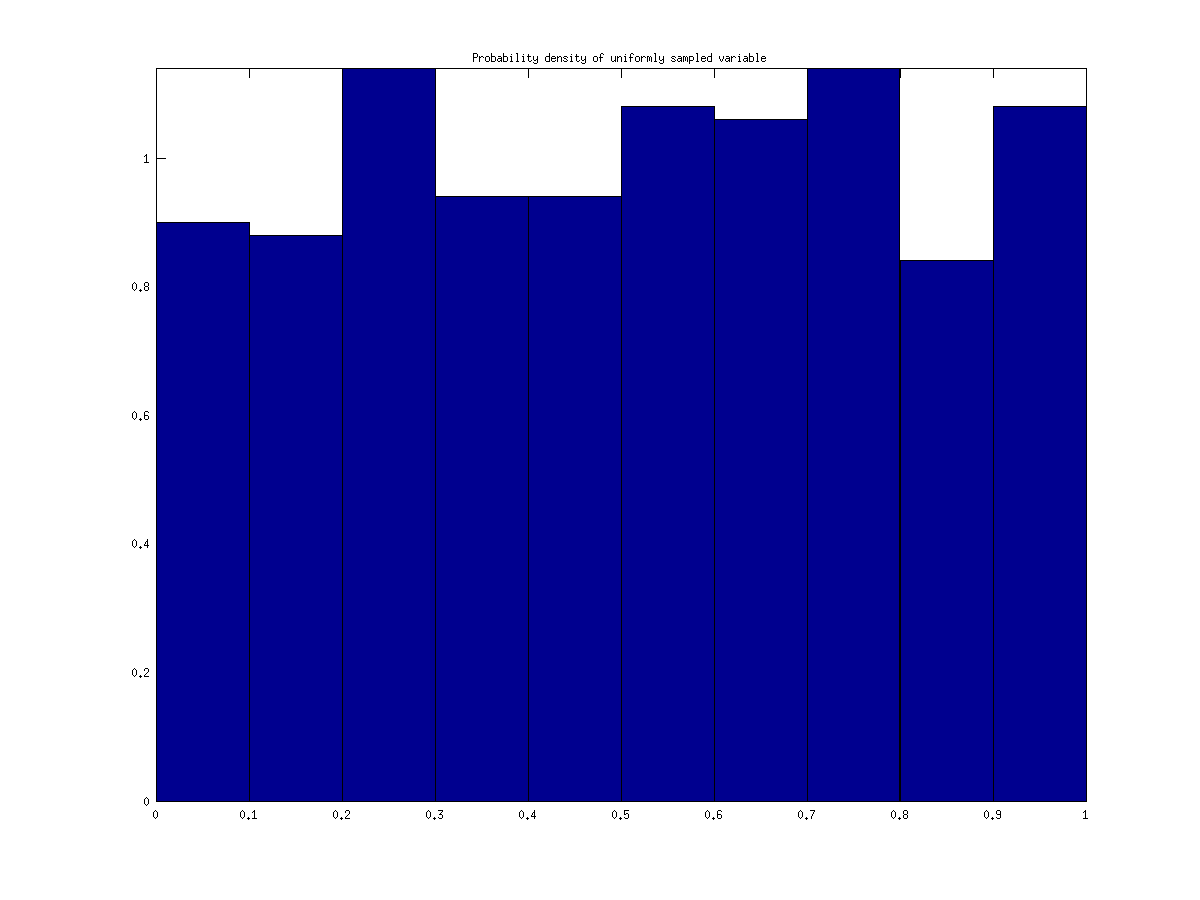
\includegraphics[width=12cm]{uniform.png}
			\caption{PDF of 500 samples}
			\label{fig:uniform}
		\end{figure}
		
		The transformed result is shown in Fig. \ref{fig:transformation}.
		\begin{figure}[H]
			\centering
			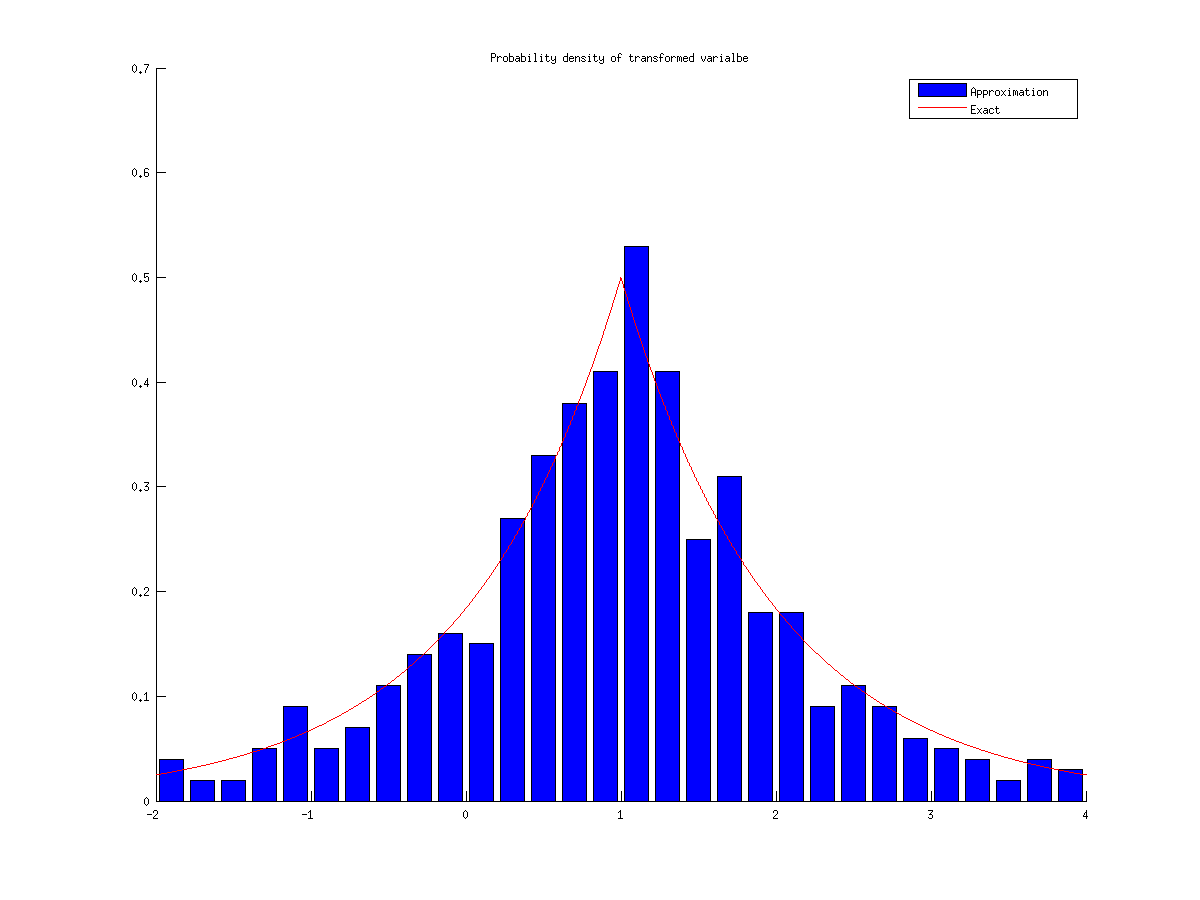
\includegraphics[width=12cm]{transformation.png}
			\caption{PDF of transformed samples and exact Laplace distribution.}
			\label{fig:transformation}
		\end{figure}
	\subsection{ICA}
		We used the constant learning rate $\eta=0.0075$ for the online natural gradient learning of the unmixing matrix.
		
		The scatter plot of the original data is given in Fig. \ref{fig:origSound}.
		\begin{figure}[H]
			\centering
			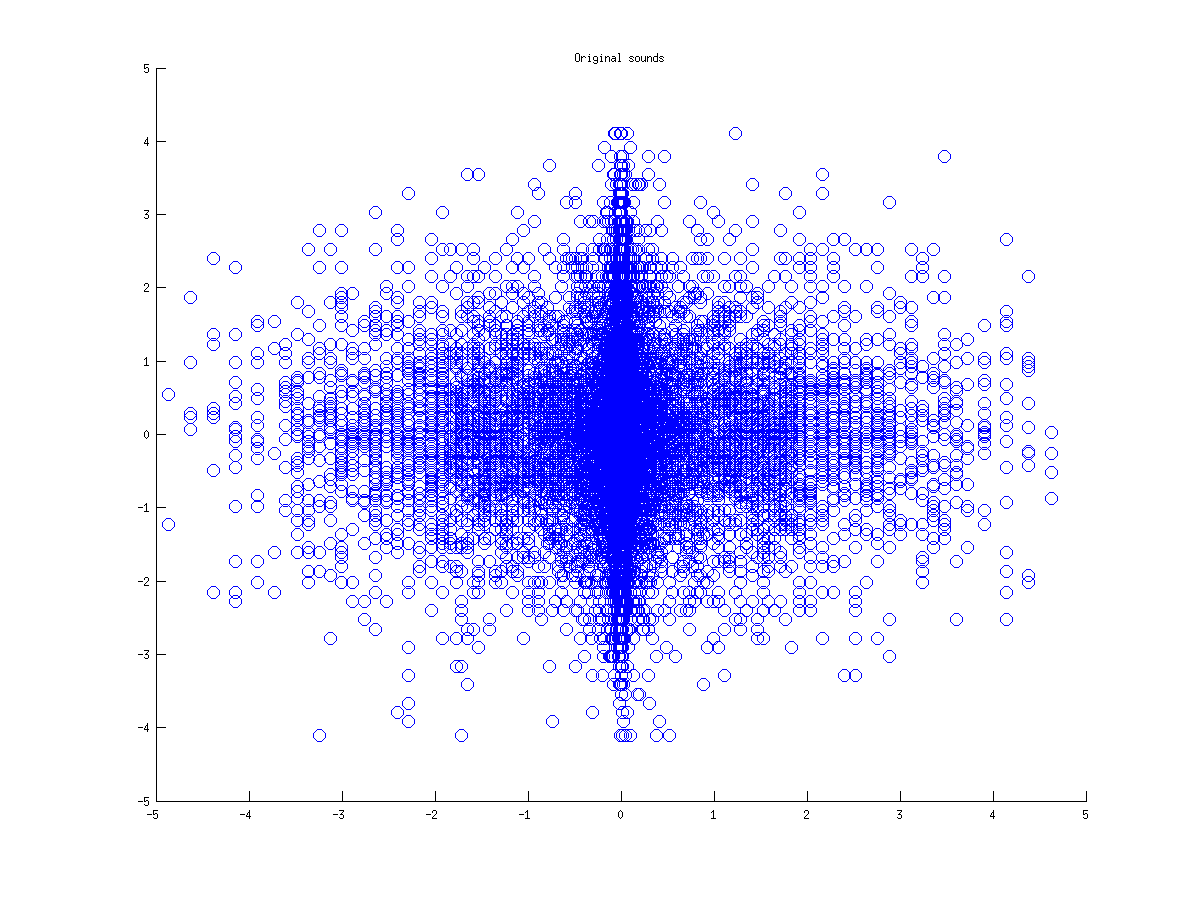
\includegraphics[width=12cm]{origSound.png}
			\caption{Scatter plot of original sound}
			\label{fig:origSound}
		\end{figure}
		
		After the mixing the data looked like in Fig. \ref{fig:mixSound}.
		\begin{figure}[H]
			\centering
			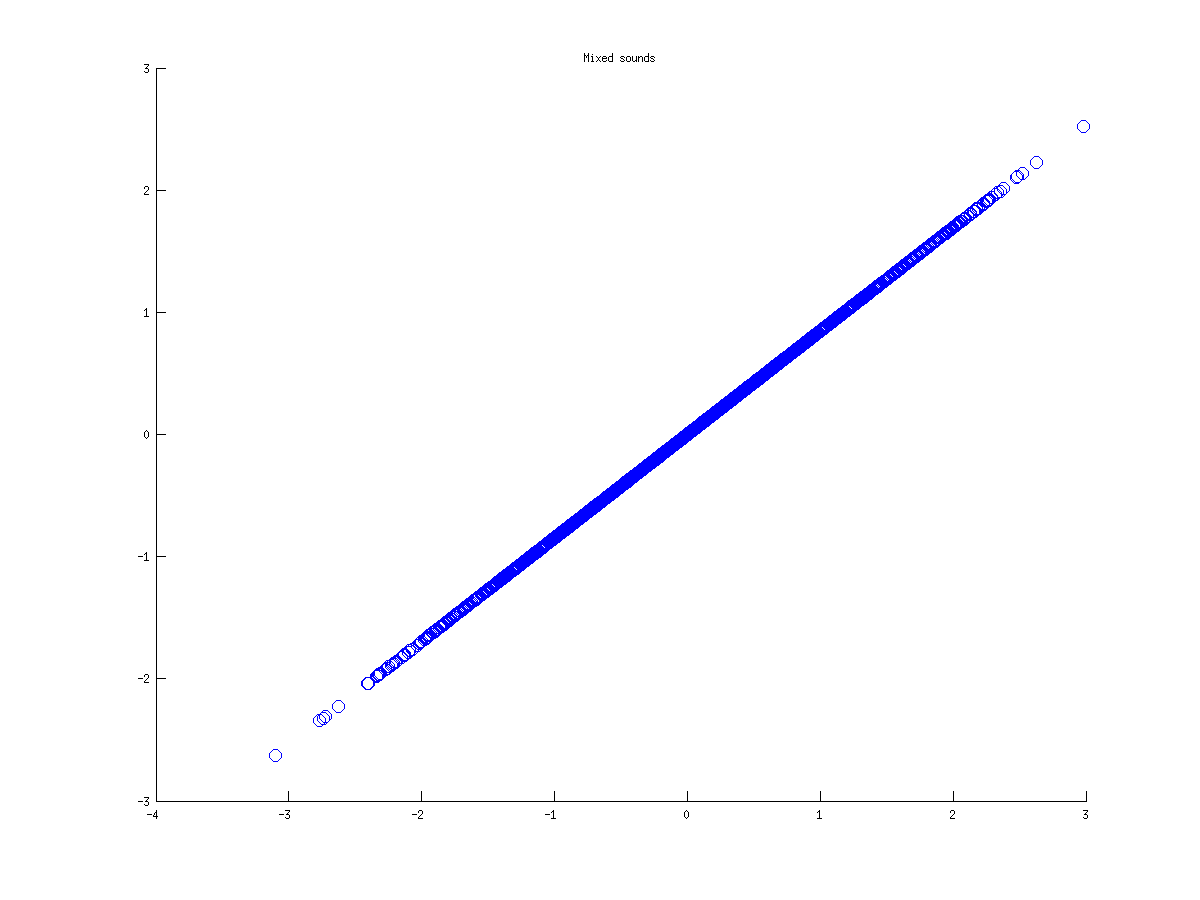
\includegraphics[width=12cm]{mixSound.png}
			\caption{Scatter plot of mixed sound}
			\label{fig:mixSound}
		\end{figure}
		
		The natural gradient learning could approximate the unmixing matrix quite well and the results are shown in Table \ref{tab:matrices}.
		\begin{table}[H]
			\centering
			\begin{eqnarray*}
				A^{-1} &=&10^3\cdot\left [
				\begin{array}{cc}
				-1.5178 & 1.7922\\
    				0.6322  &  -0.7444
				\end{array}\right]\\
				W &=&10^3 \cdot \left[
				\begin{array}{cc}
				 1.0756  & -1.2661\\
   				-2.7963   & 3.3018
				\end{array} \right]
			\end{eqnarray*}
			\caption{Original and approximated unmixing matrix}
			\label{tab:matrices}
		\end{table}
		
		The scatter plot of the recovered data is given in Fig. \ref{fig:recSound}
		\begin{figure}[H]
			\centering
			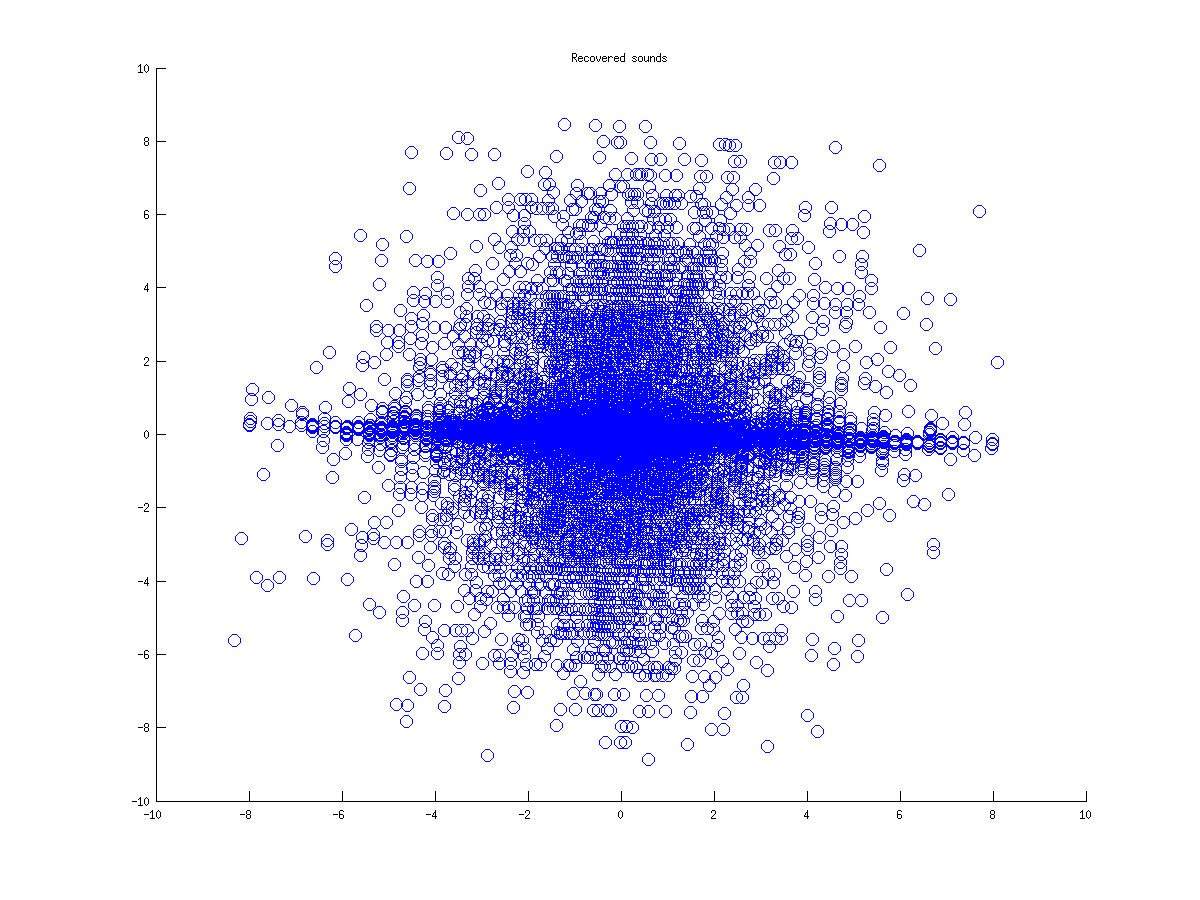
\includegraphics[width=12cm]{recSound.png}
			\caption{Scatter plot of recovered sound}
			\label{fig:recSound}
		\end{figure}
		
		The signals plotted over the time can be found in Fig. \ref{fig:soundSignal}.
		\begin{figure}[H]
			\centering
			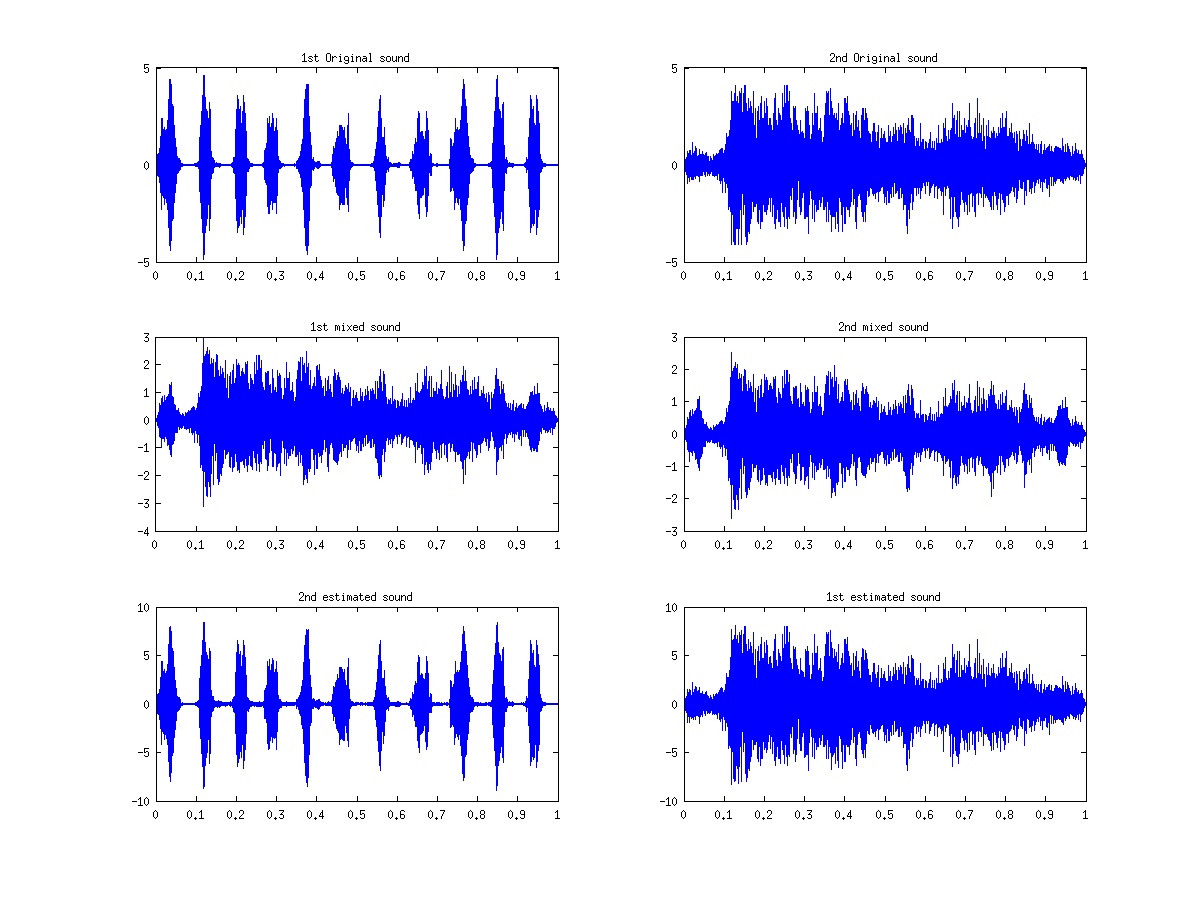
\includegraphics[width=16cm]{soundSignal.png}
			\caption{Plot of original, mixed and recovered sounds}
			\label{fig:soundSignal}
		\end{figure}
		
		As one would expect, the plot of the permutated mixed signals looks like white noise and is shown in Fig. \ref{fig:mixed1} and Fig. \ref{fig:mixed2}.
		\begin{figure}[H]
			\centering
			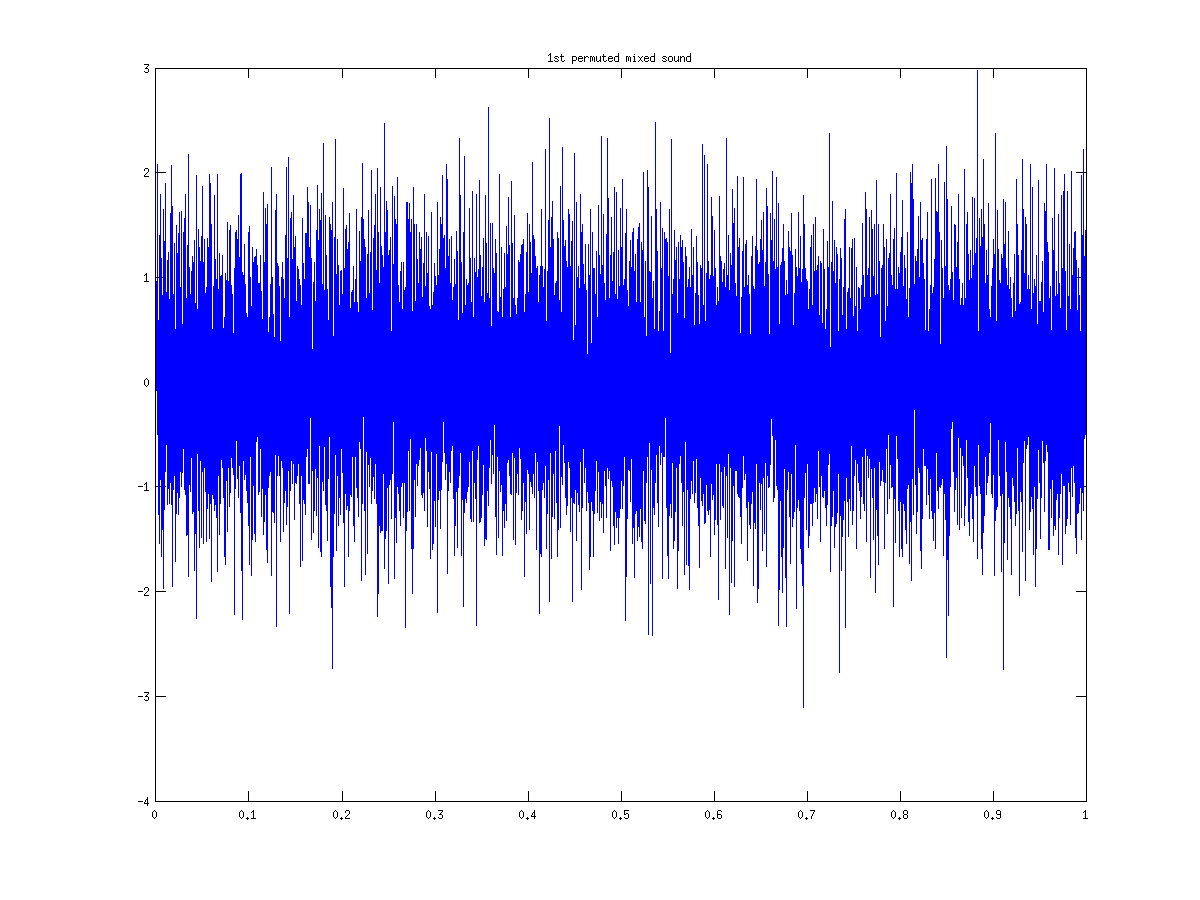
\includegraphics[width=10cm]{mixed1.png}
			\caption{Plot of 1st mixed and permutated data}
			\label{fig:mixed1}
		\end{figure}
		\begin{figure}[H]
			\centering
			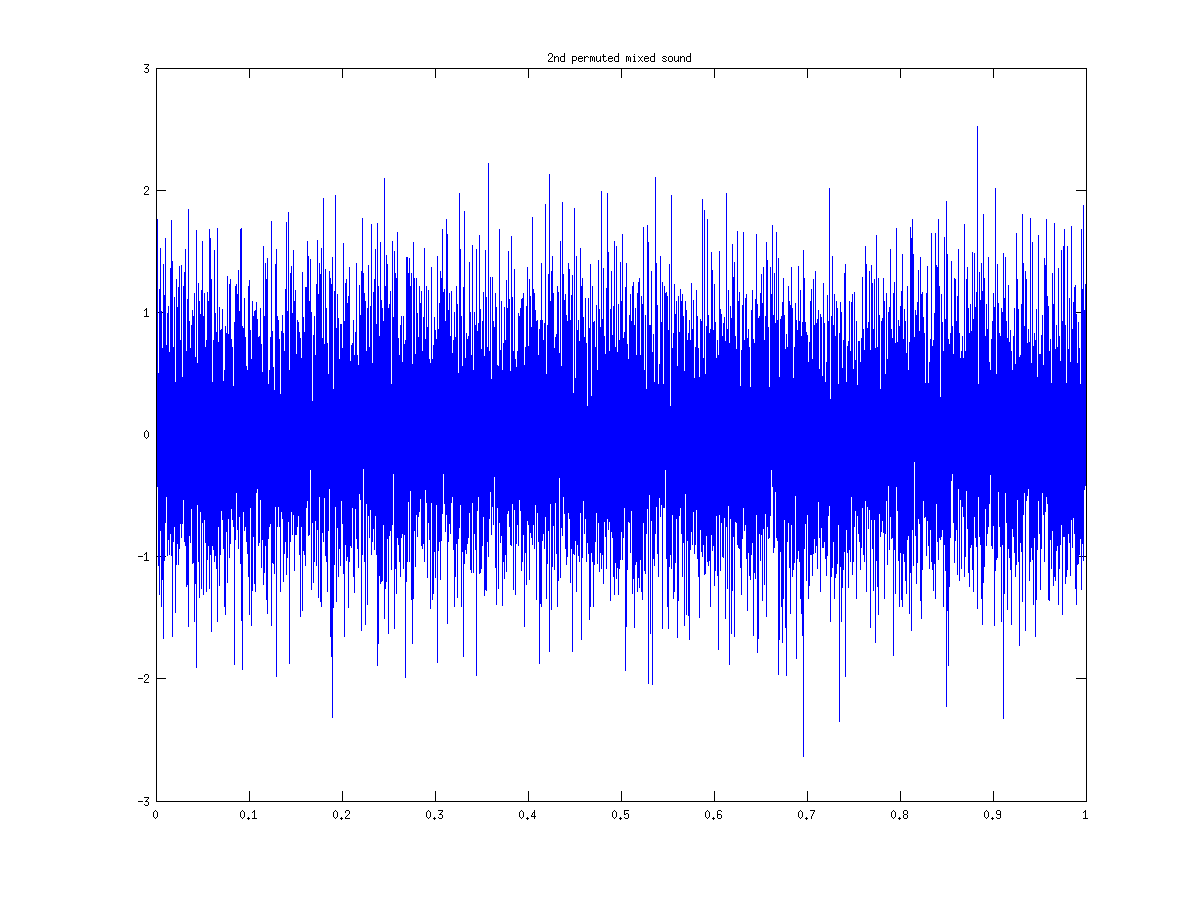
\includegraphics[width=10cm]{mixed2.png}
			\caption{Plot of 2nd mixed and permutated data}
			\label{fig:mixed2}
		\end{figure}
		
		Finally, the correlation coefficients scaled to the range $[-1,1]$ are shown in Fig. \ref{fig:correlation}.
		\begin{figure}[H]
			\centering
			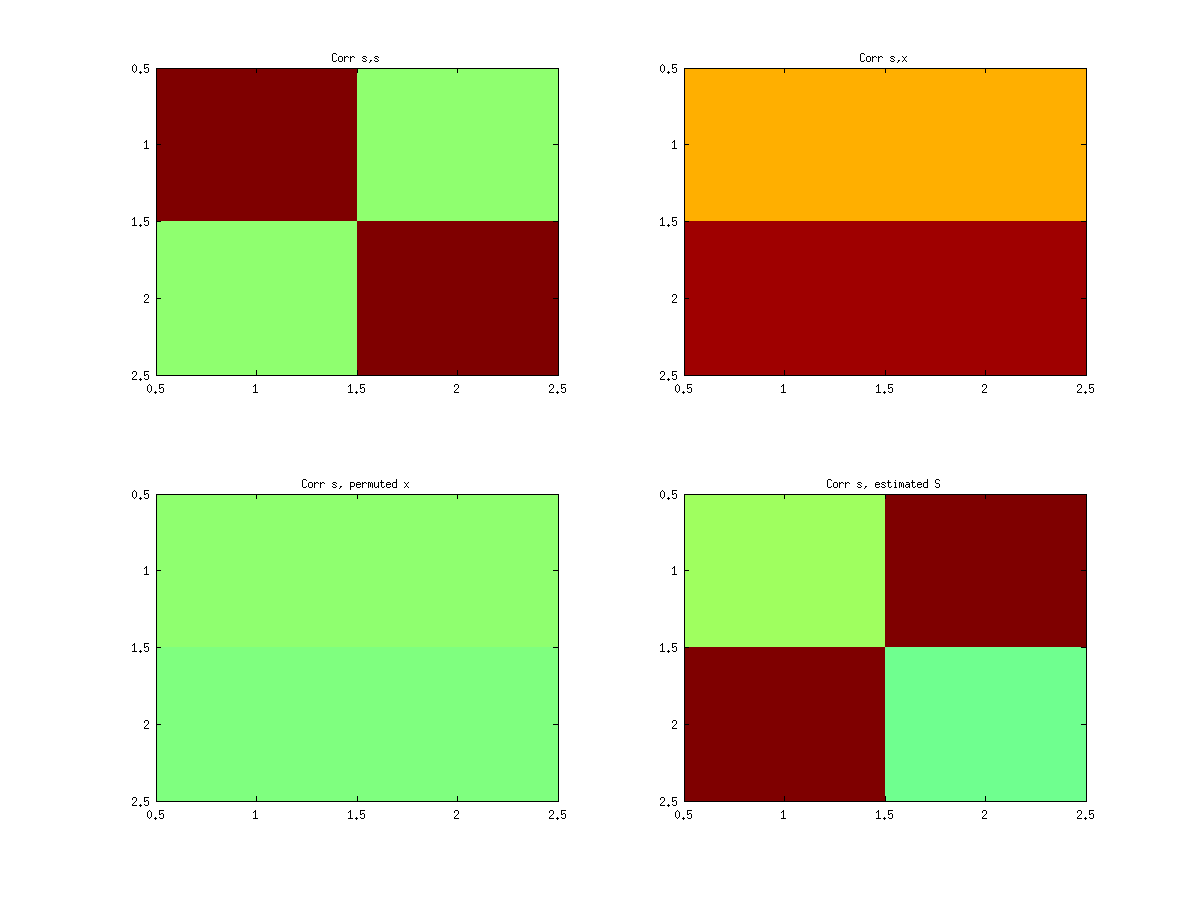
\includegraphics[width=12cm]{correlation.png}
			\caption{Top left: Correlation of original data and original data. Top right: Correlation of original data and mixed data. Bottom left: Correlation of original data and mixed and permutated data. Bottom right: Correlation of original data and recovered data.}
			\label{fig:correlation}
		\end{figure}
		
\end{document}
